\subsection{Database Generation with \emph{xsd2db}}
\label{xsd2db}
\subsubsection{Introduction}
While manually calling the chain of open source tools described in section \ref{design} to generate the necessary JAXB objects, hibernate mappings, and SQL DDL (an import file set) for each different type of XML source we wanted to import was possible.   We decided that this would violate our pattern of reusability.  It was obvious that to even build our sample application GenMAPP builder would require us to be able to import from two different XML sources, Uniprot and GO.   Thus, it was clear that it would be in the best interest of the project to create a metatool for generating these import file sets.  It is this tool that became \emph{xsd2db}.
    
\subsubsection{Design and Implementation}
Initially \emph{xsd2db} took the form of an ant build script in the original \xmlpipedb~ project.  However, as we began to add use cases to \emph{xsd2db}, most notably being able to download an XML schema,  it was decided that an executable jar would need to be built for the project.  Thus, we decided to build \emph{xsd2db} in two parts.  A command line interface, Xsd2dbCommandLine.class, and the functional component, Xsd2db.class.  These components would be kept loosely coupled i.e. the only knowledge they would have of each other is that  the \emph{xsd2db} functional component would contain a run method that could be called by the command line interface.  This way the \emph{xsd2db} functional component would be easy to integrate into future application's.

Xsd2db was created as a command line tool.  The reason behind this choice was that \emph{xsd2db} was primarily intended to be a metatool to aid developers in creating there own import engines for specific XML data.  Since our primary target is experienced users we felt that a command line interface was more appropriate than a graphical user interface and would allow us to spend more time working on the functionality of the program.    

The use case requirements for the \emph{xsd2db} functional component were many.  From start to finish \emph{xsd2db} would have several tasks it needed to complete.  First it would need to download a schema file from a user supplied URL.  It would then need to use the JAXB bindings compiler to create JAXB objects for the schema.  Next it would have to invoke the \hyperjaxb2~ add-on to generate hibernate mappings for the generated JAXB objects.  Using these hibernate mappings a SQL DDL file would then be created by using the hibernate schema export tool.  Finally, a project directory structure would need to be built to copy the generated files into, and  a build file would be generated for the project.  A UML use case diagram can be seen below in figure \ref{xsd2dbUMLUseCase}.

\begin{figure}[htbp]
\begin{center}
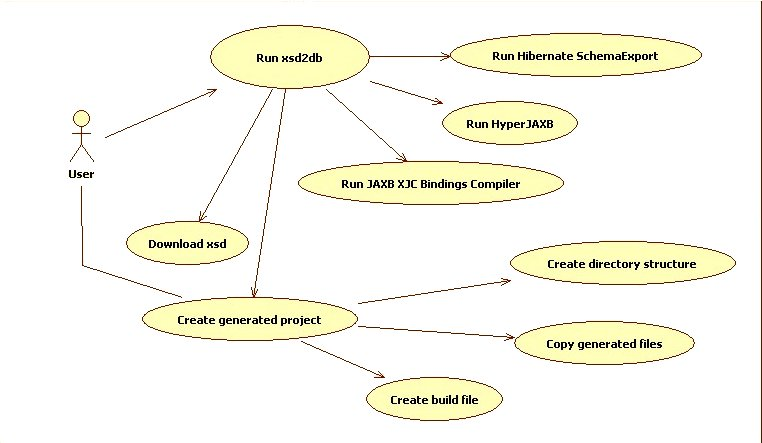
\includegraphics[scale=0.5]{./Images/xsd2dbUseCase.jpg}
\caption{Use case diagram for \emph{xsd2db}}
\label{xsd2dbUMLUseCase}
\end{center}
\end{figure}
To call the JAXB bindings compiler one must first create a  com.sun.tools.xjc.Options object.  One can then use the Options object to set the target directory for generated JAXB object files, the schema type of the XML schema (DTD or XSD), and finally the location of the schema to be parsed.  Once the Options object is configured you can annotate the schema and create an annotated grammar by invoking the com.sun.tools.xjc.GrammarLoader.load()  factory method on the Options object and an ErrorReceiver object.  An ErrorReceiver is simply an object that implements the com.sun.tools.XJC.ErrorReceiver interface and allows a developer to decided how to handle errors;  in our case we simply reported them to the command line.   Once you have created an annotated grammar the XJC bindings compiler can be invoked using the static method Driver.generateCode() method on the AnnotatedGrammer, XJC Options object, and the ErrorReciver.  Some sample code is shown in figure \ref{XJCsamplecode}.
\begin{figure}[htbp]
\begin{center}
\begin{verbatim}     
        ErrorReceiver errorReceiver = new ErrorReceiverImpl();
        AnnotatedGrammar grammar = null;
        try {
            // Create a annotated grammar
            grammar = GrammarLoader.load(XJCOptions, errorReceiver);
            if (grammar == null)
                System.out.println("Unable to parse schema");
        } catch(Exception e) {
            System.out.println("Error loading the grammar");
            e.printStackTrace(); 
        }
        try {
            // Generate the JAXB objects
            GeneratorContext generatorContext;
            generatorContext = Driver.generateCode(
                 grammar, 
                 XJCOptions, 
                 errorReceiver);
            if (generatorContext == null)
                System.out.println("failed to compile a schema");
          }
        
\end{verbatim}

\caption{Code to invoke the JAXB XJC bindings compiler.}
\label{XJCsamplecode}
\end{center}
\end{figure}

To invoke the \hyperjaxb2~ add-on we take advantage of the fact that all JAXB add-ons must provide a run method since they implement the JAXB AbstractParameterizableCodeAugmenter interface.  Thus to create the hibernate mapping files for the generated JAXB objects, we create a new Hyperjaxb2 add-on and call run using the AnnotatedGrammar, GeneratorContext,  and XJC Options Objects that we created while invoking the XJC bindings compiler. 

In order to generate the SQL DDL file we use the Hibernate SchemaExport object.  Hibernate requires that the Hibernate Configuration object be created and configured before any hibernate objects can be used.  To configure the Hibernate Configuration object we simply load an included Hibernate properties file and use the Hibernate Configuration object's setProperties() method to configure Hibernate.  The last step of the Hibernate Configuration is to inform Hibernate of the location of the Hibernate mapping files that it will be using.  In \emph{xsd2db} we decided to do this manually using the Configuration object's addFile() method.   Once hibernate is configured, generating a SQL DDL file is very simple.  All we must do is create a new SchemaExporter, set the output directory for the DDL file, set the delimiter for the DDL file, and finally create the DDL file by calling the create() method on the SchemaExporter.  Sample code can be seen in figure \ref{schemaExportSampleCode}.
\begin{figure}[htbp]
\begin{center}
\begin{verbatim}
         // Initialize hibernate
        hibernateConfig = new Configuration();
        File hibPropertiesFile = new File(HIB_PROPERTIES);
        Properties hibProperties = new Properties();
        try {
            hibProperties.load(new FileInputStream(hibPropertiesFile));
        } catch(Exception e) {
            System.out.println("Properties file failed to load.");
        }
        hibernateConfig.setProperties(hibProperties);

         // Add a hibernate mapping file
         hibernateConfig.addFile(hbmMappingFile);
         
        // Produce the SQL file.
        SchemaExport schemaExporter = new SchemaExport(hibernateConfig);
        schemaExporter.setOutputFile(fullOutputPath);
        schemaExporter.setDelimiter(";");
        schemaExporter.create(true, false);
\end{verbatim}
\caption{Schema export sample code}
\label{schemaExportSampleCode}
\end{center}
\end{figure}

The Last phase of \emph{xsd2db} is to create a standalone project that is ready to be compiled using Ant.  To this end we first create a project directory structure. The directory structure produced is shown in figure \ref{xsd2dbStructure}.  We then copied the necessary library files needed to compile the generated project from the lib directory of \emph{xsd2db} to the lib directory of the generated project.  Finally we generate a build file using a canned build file that we included as a resource in the \emph{xsd2db} jar.   

\begin{figure}[htbp]
\begin{center}
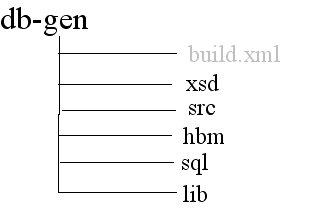
\includegraphics[scale=0.8]{./Images/xsd2dbStructure.jpg}
\caption{{\bf \emph{xsd2db}output project directory structure}}
\label{xsd2dbStructure}
\end{center}
\end{figure}

After this last phase the user can then compile the output of \emph{xsd2db} using the generated build file.  The resultant out put is a java library file that can be combined with the \emph{xmlpipedbutils} described in section \ref{xmlpipedbutils} to create a functional application capable of importing data from the user's XML sources and to a relational database and querying that database.

\subsubsection{Performance Analysis}
\emph{xsd2db} has been tested on three different XML schema files with varying degrees of success.  We preformed initial testing on the Books.xsd schema.  Books.xsd is the canonical schema used in most example applications that use XML data and thus we felt it was an appropriate choice for our initial test schema.  When using \emph{xsd2db} we were able to import XML data into a Postgresql database, and later query that database without making any modifications to our generated files.  The success of this initial test lead us to try using \emph{xsd2db} on two other schemas: Uniprot.xsd and the GO DTD schema.  

After running \emph{xsd2db} on the Uniprot.xsd we discovered that some post processing would be required on the generated project before we would be able to import XML data into a Postgresql database.  This was largely due to several incompatiblities with the Postgresql database and no fault of \emph{xsd2db}.  However, one problem did arise which was a direct occurance of a failure of \emph{xsd2db} to properly handle XSD union types.  This was later attributed to a bug in \hyperjaxb2~  and remains a part of \emph{xsd2db}.  We created another tool, uniprotdb, to resolve these issues by post processing the output of \emph{xsd2db}.  A more thorough examination of these problems as well as a detailed description of uniprotdb can be found in section \ref{uniprotdb}.

The last schema file we tested \emph{xsd2db} on was the GO schema file.  The GO schema file presented a unique challenge in that it differed from the other schemas we tested \emph{xsd2db} on since it was DTD and not an XSD schema.  Again as with the Uniprot.xsd we encounter some problems with Postgresql and had to develop a post processor for GO, \emph{godb}.  \emph{godb} and the problems we encountered are described in more detail in section \ref{godb}.

In addition to the test we preformed with these three different schemas \emph{xsd2db} also contains several unit test of the command line interface.  Thus, we are sure that the command line interface works and is bug free.

Overall it can be said, that \emph{xsd2db} does what is intended.  It is a metatool for developers to create there own xml import engines, thus it is reasonable that it might require post processing depending on a developer's design choices.  However, despite this initial success it is clear that there remains work to be done to improve the performance and robustness of \emph{xsd2db}. 

\subsubsection{Future Work}
For the first round of development we initially focused on simply getting \emph{xsd2db} working as quickly as possible.  While some minor unit testing has been preformed, as well as, a good amount of maintenance to re-factor the code base, more can always be done.  

One aspect we would like to work on would be to improve the compatibility of \emph{xsd2db} with the Postgresql database.  This would fix  the problems with both biological databases referenced in sections \ref{uniprotdb} and \ref{godb}.  In addition, on the same line of thought we would like to fix the XSD union bug in \hyperjaxb2.

Another area of improvement in \emph{xsd2db} would be to develop more unit test for both the \emph{xsd2db} command line and the \emph{xsd2db} functional unit.  When the unit test were initially written for xsd2db the functional component was not written in a state that would lend itself to be easily unit tested.  It has since been re-factored and unit test should be written.

The last area of improvement, would be to possibly add a graphical interface to \emph{xsd2db}.  While \emph{xsd2db} is primarily intended as a tool for developers and thus a command line interface is appropriate, adding a graphical interface to \emph{xsd2db} can only ease its use.



